%%%%%%%%%%%%%%%%%%%%%%%%%%%%%%%%%%%%%%%%%%%%%%%%%%%%%%%%%%%%%%%%%%%%%%%%%%%%%%%%
% Introduction
%%%%%%%%%%%%%%%%%%%%%%%%%%%%%%%%%%%%%%%%%%%%%%%%%%%%%%%%%%%%%%%%%%%%%%%%%%%%%%%%
\subsection{Introductions}
\label{anomalyDetection:commuteTime:introduction}
This section provides an overview of a method for anomaly detection using
commute time. This method was proposed by \citeauthor{Khoa:2012} in
\fullcite{Khoa:2012} \cite{Khoa:2012}. An introduction to commute time was
presented in \autoref{commuteTime}. The method described in this section forms
the base algorithm that will be implemented in hardware during this \thesis{}.

Commute time is an Euclidean distance in the space spanned by eigenvectors of
the graph Laplacian matrix. Commute time forms an interesting basis for an
anomaly detection algorithm because, unlike traditional Euclidean distance,
the commute time between two nodes can capture both the distance between them
and the data densities so that we can capture both global and local anomalies in
the data set \cite{Khoa:2012}.

% TODO: Replace with a tikzpicture
\begin{figure}
    \centering
    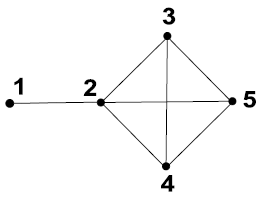
\includegraphics[width=0.3\textwidth]{commute-time/example}
    \caption{A simple example illustrating the application of commute time
        \cite{Khoa:2012}}
    \label{fig:commuteTime:example}
\end{figure}

A simple example illustrating the application of the commute time metric is
shown in \autoref{fig:commuteTime:example}. In this example, edge $e_{1,2}$ has
a larger commute time than all other edges in the cluster, whilst its Euclidean
distance is the same or smaller than the neighbouring Euclidean distances.

A key property of the commute time metric that allows for its use for anomaly
detection is that, by adding more data points to an existing cluster (i.e.,
making the cluster more dense), the commute time between anomalous data points
and the cluster changes dramatically whilst the average pair-wise commute times
of all nodes within the cluster is largely unaffected. This property is
illustrated in \autoref{fig:commuteTime:example2}.

% TODO: Replace with a tikzpicture
\begin{figure}
    \centering
    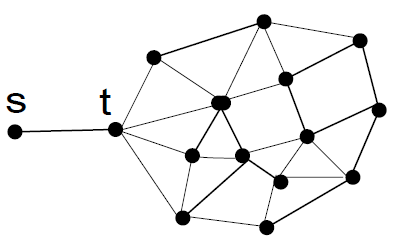
\includegraphics[width=0.3\textwidth]{commute-time/example2}
    \caption[The commute distance from an anomaly to a node in a cluster
        increases when the cluster is denser]{The commute distance from an
        anomaly ($s$) to a node in a cluster ($t$) increases when the cluster is
        denser \cite{Khoa:2012}}
\end{figure}

\citeauthor{Khoa:2012} was able to devise and prove an anomaly detection
algorithm (using the commute time metric) to detect global and local outliers.
Extending this algorithm, \citeauthor{Khoa:2012} was able to use graph component
sampling and Eigenspace approximation in order to avoid the $O(n^3)$ Eigen
decomposition of the graph Laplacian. Furthermore, a pruning technique was used
in attempt to improve the run time complexity of the algorithm to $O(n\log n)$.

%%%%%%%%%%%%%%%%%%%%%%%%%%%%%%%%%%%%%%%%%%%%%%%%%%%%%%%%%%%%%%%%%%%%%%%%%%%%%%%%
% Random Walks
%%%%%%%%%%%%%%%%%%%%%%%%%%%%%%%%%%%%%%%%%%%%%%%%%%%%%%%%%%%%%%%%%%%%%%%%%%%%%%%%
\subsection{Random Walks}
\label{anomalyDetection::randomWalks}

\cite{Khoa:2012}
While commute time is a robust measure for detecting both global and local anomalies, the main drawback is its computational time. The direct computation of commute time involves the eigen decomposition of the graph Laplacian matrix which is proportional to $O(N^3)$ and is not feasible for large graphs ($N$ is the number of nodes). In this work, the graph components are sampled to reduce the graph size and then eigenspace approximation in [60] is applied to approximate the commute time on the sampled graph.

An easy way to sample a graph is selecting nodes from it uniformly at random. However, sampling in this way can break the graph geometry structure and anomalies may not be chosen after sampling. To resolve this, we propose a sampling strategy called component sampling. After creating the mutual k1-nearest neighbour graph, the graph tends to have many connected components corresponding to different data clusters.
Anomalies are likely isolated nodes or nodes in very small components. For nodes in normal components (we have a threshold to distinguish between normal and anomalous components), they are uniformly sampled with the same ratio p = 50k1 /n, which is chosen from preliminary experimental results. For nodes in anomalous components, we leave all of them intact. Then we rebuild a mutual k1 -nearest neighbour graph for
the sampled data. Sampling in this way will maintain the geometry of the original graph and the relative densities of normal clusters. Anomalies are also not discarded in this sampling strategy.

\begin{equation}
c_{ij} = V_G(x_i - x_j)^T (x_i - x_j)
\end{equation}
Therefore, the commute time between nodes on the graph can be viewed as the
squared Euclidean distance in the node space spanned by eigenvectors of the graph
Laplacian matrix.

Denote $\tilde{V}$, $\tilde{S}$ be a matrix containing $m$ largest eigenvectors of $L^+$ and its corresponding diagonal matrix, and $\tilde{x}_i = \tilde{S}^{-1/2}\tilde{V}^Te_i$, the approximate commute time is:
\begin{equation}
\tilde{c}_{ij} = V_G(\tilde{x}_i - \tilde{x}_j)^T(\tilde{x}_i - \tilde{x}_j)
\end{equation}

The commute time $c_{ij}$ in an $n$ dimensional space is transformed to the commute time $\tilde{c}_{ij}$ in an $m$ dimensional space. Therefore, we just need to compute the $m$ smallest eigen-vectors with nonzero eigenvalues of $L$ (i.e.\ the largest eigenvectors of $L^+$) to approximate the commute time.

%%%%%%%%%%%%%%%%%%%%%%%%%%%%%%%%%%%%%%%%%%%%%%%%%%%%%%%%%%%%%%%%%%%%%%%%%%%%%%%%
% Anomaly Detection Using Commute Time
%%%%%%%%%%%%%%%%%%%%%%%%%%%%%%%%%%%%%%%%%%%%%%%%%%%%%%%%%%%%%%%%%%%%%%%%%%%%%%%%
\subsection{Anomaly Detection Using Commute Time}
\label{anomalyDetection:commuteTime:algorithm}
The algorithm proposed by \citeauthor{Khoa:2012} in \fullcite{Khoa:2012}
\cite{Khoa:2012} is presented in \autoref{algm:anomalyDetection:commuteTime}.
This section describes in detail each stage of the algorithm.

\begin{algorithm}[t]
    % TODO
\LinesNumbered

\SetKwInput{InputK}{k}
\SetKwInput{InputN}{N}
\SetKwInput{InputD}{Data}
\SetKwInOut{OutputO}{outliers}

\InputK{the number of nearest neighbors}
\InputN{the number of outliers to return}
\InputD{a set of examples in random order}
\OutputO{a set of outliers}

\SetKwData{varB}{b}
\SetKwData{Block}{block}
\SetKwData{Cutoff}{cutoff}
\SetKwData{varD}{d}
\SetKwData{Data}{Data}
\SetKwData{varK}{k}
\SetKwData{varN}{N}
\SetKwData{Neighbours}{neighbours}
\SetKwData{varO}{o}
\SetKwData{Outliers}{outliers}
\SetKwData{Score}{score}

\SetKwFunction{Closest}{closest}
\SetKwFunction{Distance}{distance}
\SetKwFunction{GetNextBlock}{getNextBlock}
\SetKwFunction{MaxDist}{maxDist}
\SetKwFunction{Min}{min}
\SetKwFunction{Top}{top}

\Begin{
    $\Cutoff \longleftarrow 0$\tcp*[l]{set the cutoff for pruning to $0$}
    $\Outliers \longleftarrow \emptyset$\tcp*[l]{initialize to the empty set}
    \BlankLine
    \While(\tcp*[h]{load a block of examples from \varD}){$\Block \longleftarrow \GetNextBlock{\Data}$}{
        $\Neighbours(\varB) \longleftarrow \emptyset, \quad \forall \, \varB \in \Block$\;
        \BlankLine
        \ForEach{$\varD \in \Data$}{
            \ForEach{$\varB \in \Block \: : \: \varB \neq \varD$}{
                \If{$|\Neighbours(\varB)| < \varK \: \lor \: \Distance{\varB, \varD} < \MaxDist{\varB, \Neighbours(\varB)}$}{
                    $\Neighbours(\varB) \longleftarrow \Closest{\varB, \Neighbours(\varB)} \cup \varD, \varK)$\;
                    \If{$\Score(\Neighbours(\varB), \varB) < \Cutoff$}{
                        $\Block \longleftarrow \Block \setminus \varB$\;
                    }
                }
            }
        }
        \BlankLine
        $\Outliers \longleftarrow $\Top{$\Block \cup \Outliers$, $\varN$}\tcp*[l]{keep only the top n outliers}
        $\Cutoff \longleftarrow \Min_{\varO \in \Outliers}(\Score(\varO))$\tcp*[l]{the cutoff is the score of the weakest outlier}
    }
    \KwRet{\Outliers}\;
}

    \caption{Anomaly detection using commute time}
    \label{algm:anomalyDetection:commuteTime}
\end{algorithm}

% Construction of the k-Nearest Neighbour Graph
\subsubsection{Construction of the $k$-Nearest Neighbour Graph}
\label{anomalyDetection:commuteTime:algorithm:knnGraph}
The first stage of the algorithm is to compute the $k$-nearest neighbour graph
for the input data set.

For this purpose, the $kd$-tree technique can be applied so as to avoid an
$O(n^2)$ searching of nearest neighbours.

Algorithm
The proposed method is outlined in Algorithm 3. We create the sampled graph from the data using graph components sampling. Then the graph Laplacian $L_s$ of the sampled graph and matrix $\tilde{V}$ ($m$ smallest eigenvectors with nonzero eigenvalues of $L_s$) are computed. Since we use the pruning technique, we do not need to compute the approximate commute time for all pairs of points. Instead, we compute it `on demand'.

Algorithm 3: Commute Time Distance Based Anomaly Detection with Graph
Component Sampling and Eigenspace Approximation.
Input: Data matrix X, the numbers of nearest neighbours k1 and k2, the numbers
of anomalies to return N
Output: Top N anomalies
1: Construct the mutual k1-nearest neighbour graph from the dataset
2: Do the graph component sampling
3: Reconstruct the mutual k1-nearest neighbour graph from sampled data
4: Compute the Laplacian matrix of the sampled graph and its m smallest
eigenvectors
5: Find top N anomalies using the commute time based technique with pruning rule
(using k2)
6: Return top N anomalies

The $k$-nearest neighbour graph with $n$ nodes is built in $O(n \log n)$ using kd-tree with the assumption that the dimensionality of the data is not very high. The average degree of each node is $O(k)$ ($k << n$). So the graph is sparse and thus finding connected components take $O(kn)$. After sampling, the size of graph is $O(n_s)$ ($n_s << n$). The standard method for eigen decomposition of $L_s$ is $O({n_s}^3$. Since $L_s$ is sparse, it would take $O(Nn_s) = O(k{n_s}^2$ where $N$ is the number of nonzeros. The computation of just the $m$ smallest eigenvectors ($m < n_s$) is less expensive than that.

The typical distance-based anomaly detection takes $O({n_s}^2$) for the neighbourhood search. Pruning can scale it nearly linear [5]. We only need to compute the commute times $O(n_s)$ times each of which takes $O(m)$. So the time needed for two steps is proportional to $O(n \log n + kn + k{n_s}^2 + mn_s = O(n \log n)$, as $n_s << n$.